\section{Results}

\textit{Model, physical hierarchy, and exact authority.---}
The single-particle sector is
$h(k)=t\cos k\,\sigma_0+\lambda_y\sin k\,\sigma_y+[\lambda_z\sin k+J_A\cos k]\sigma_z$.
The odd-in-$k$ spin-orbit fields and the altermagnetic $J_A\cos k$ splitting produce a momentum-dependent spin texture, while pairing connects states shifted by $\pm q/2$ in the Nambu Hamiltonian.  A finite-momentum state therefore cannot be found by optimizing the order-parameter amplitude alone: for every external coordinate $x$ the exact oracle determines
\begin{equation}(\Delta_{\rm opt},q_{\rm opt})=\operatorname*{arg\,min}_{\Delta,q}F_{\rm impl}(\Delta,q),\end{equation}
where $F_{\rm impl}$ is the normal-referenced occupation-weighted spectral objective used by the implemented numerical calculation.  Its reliable minimum gives Normal order when the optimum is unpaired, uniform superconductivity when $\Delta_{\rm opt}>0$ and $q_{\rm opt}$ is zero within resolution, and FFLO order when both the amplitude and finite momentum are resolved.

\begin{figure*}[tbp]
\centering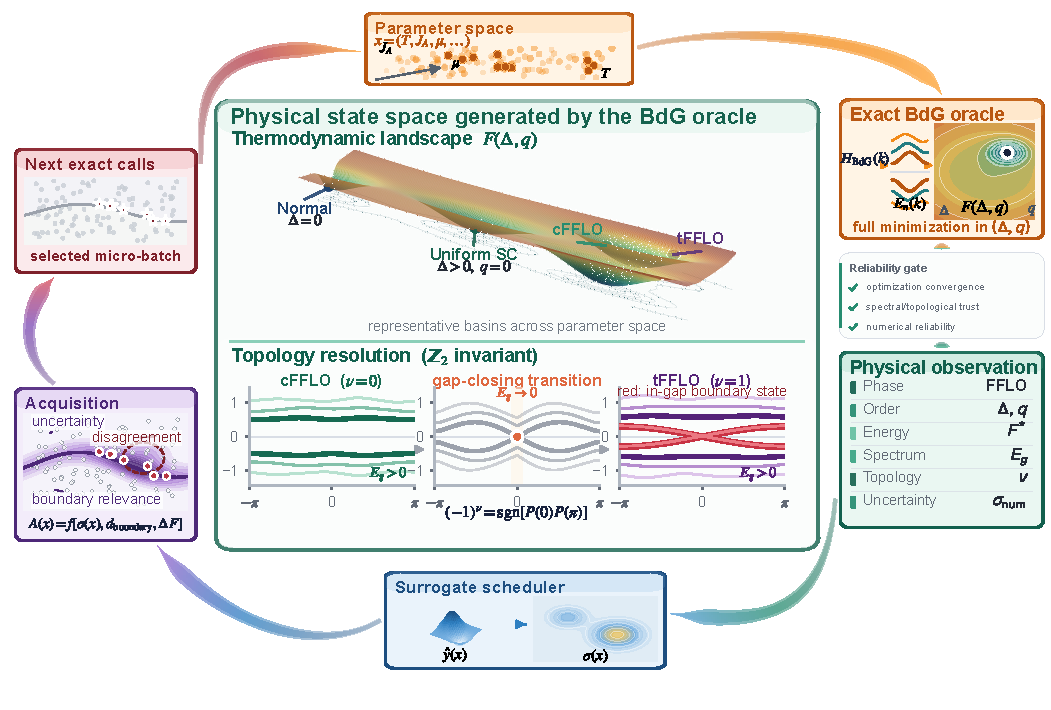
\includegraphics[width=0.96\textwidth]{figures/Fig1_candidate.pdf}
\caption{\textbf{Physical hierarchy and adaptive scheduling.} The altermagnetic and spin-orbit BdG model generates a normal-referenced $F_{\rm impl}(\Delta,q)$ landscape. Its reliable minimum determines Normal, uniform-SC, or FFLO order; only a gapped FFLO minimum proceeds to the Pfaffian test. The surrogate cycle proposes subsequent exact calls and does not determine either label.}
\label{fig:framework}\end{figure*}

Topology is a second, logically separate test.  It is evaluated only for a thermodynamically accepted, numerically reliable FFLO minimum whose full Brillouin-zone spectrum is gapped.  Under that applicability condition,
\begin{equation}(-1)^\nu=\operatorname{sgn}[P(0)P(\pi)]\end{equation}
distinguishes cFFLO ($\nu=0$) from tFFLO ($\nu=1$); a change of index requires a bulk gap closing and reopening, not a change in basin depth or the sign of $q$.  Figure~\ref{fig:framework} summarizes this hierarchy.  Regression and classification ensembles see accepted exact observations and rank the next microbatch, but every physical label remains an output of the BdG objective and spectral tests.

\FloatBarrier

\textit{Two-dimensional thermodynamic organization.---}
The exact observations in Fig.~\ref{fig:thermo} organize into a curved outer envelope separating superconducting support below from Normal support above.  At low temperature the superconducting sector reaches comparatively large $J_A/t$; as temperature rises, the largest sampled splitting that still supports pairing moves downward.  Most of the paired region is finite-$q$ FFLO.  Uniform superconductivity instead forms a narrow strip close to $J_A=0$, so the sampled state changes rapidly from zero- to finite-momentum pairing once the altermagnetic splitting is introduced.  This thin inner structure and the descending outer envelope are precisely the regions where small changes of the optimized minimum can change a label, motivating concentrated exact minimization rather than a smooth surrogate boundary.

\begin{figure}[tbp]
\centering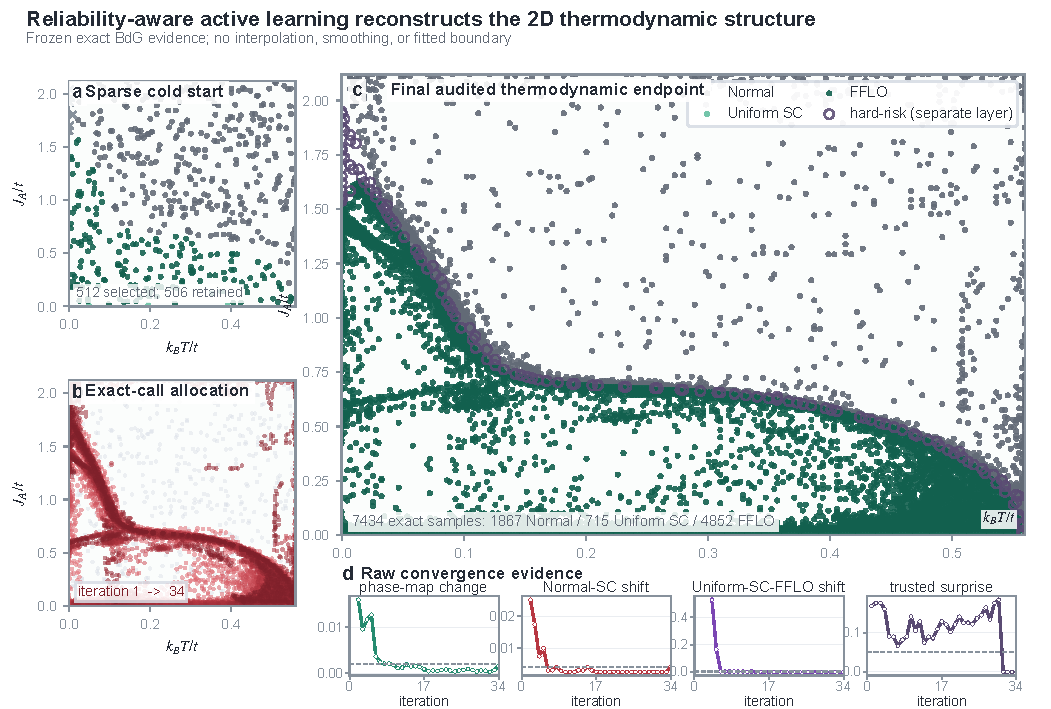
\includegraphics[width=0.98\columnwidth]{figures/Fig2_candidate.pdf}
\caption{\textbf{Two-dimensional thermodynamic reconstruction.} \textbf{(a)} Sparse exact initialization. \textbf{(b)} Exact-call allocation across the Stage-I discovery and Stage-II reliability continuation. \textbf{(c)} The 7,434-coordinate Stage-II endpoint, which contains the 6,880-coordinate Stage-I endpoint plus 554 additional exact coordinates; open symbols denote numerically flagged evaluations, not a phase. \textbf{(d)} Numerical histories. The 8.89\% and 11.24-fold headline refer specifically to the Stage-I endpoint and prescribed candidate grid.}
\label{fig:thermo}\end{figure}

The search begins with a sparse random design over the full $(k_BT/t,J_A/t)$ domain.  Subsequent calls accumulate along both thermodynamic structures while a continuing exploration channel samples their interiors and the remaining domain.  In the primary Stage-I discovery, 6,880 unique exact coordinates are retained from 77,361 prescribed candidate locations, corresponding to an 8.89\% location fraction and an 11.24-fold reduction relative to evaluating every grid location.  The Stage-II reliability continuation adds exact evaluations without changing any shared phase label and supplies the 7,434-coordinate endpoint shown in panel (c).  The efficiency ratio is therefore a Stage-I location count, not a wall-time acceleration or a comparison with matched random sampling.

\FloatBarrier

\textit{Topology-resolved FFLO structure.---}
Thermodynamic FFLO order alone does not specify the bulk topological sector.  Applying the full-zone gap guard and Pfaffian invariant resolves the trusted FFLO observations into two gapped supports (Fig.~\ref{fig:topology}).  The cFFLO sector occupies lower $J_A/t$ and extends to higher temperature, whereas the sampled tFFLO sector is shifted toward stronger altermagnetic splitting and lower temperature.  Their meeting region follows a curved locus where the bulk gap closes before reopening with the opposite Pfaffian product.  Thus the topology-resolved map adds a bulk-state distinction that neither the position of the $F_{\rm impl}$ minimum nor the sign of $q_{\rm opt}$ can provide.

\begin{figure}[tbp]
\centering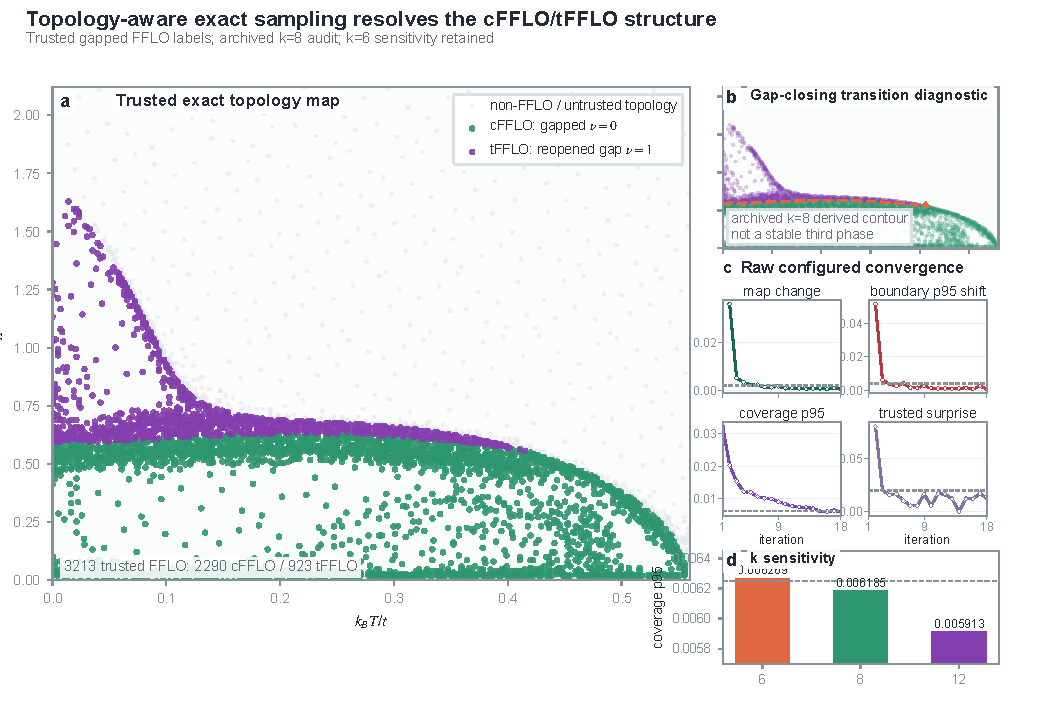
\includegraphics[width=0.98\columnwidth]{figures/Fig3_candidate.pdf}
\caption{\textbf{Bulk topology inside the thermodynamic FFLO sector.} \textbf{(a)} Trusted gapped FFLO observations resolved into cFFLO and tFFLO by the full-zone gap and Pfaffian invariant. \textbf{(b)} A support-restricted contour and local opposite-$\mathbb Z_2$ brackets locate a gap-closing region but not an exact boundary. \textbf{(c,d)} Numerical histories and neighborhood sensitivity are retained in the artwork; their detailed values are reported in the Supplemental Material.}
\label{fig:topology}\end{figure}

The exact labels are discrete, so the plotted transition line is a support-restricted reconstruction rather than an independently calculated phase boundary.  Nearby observations with opposite $\mathbb Z_2$ indices bracket the transition region, and changing the reconstruction neighborhood produces a finite displacement of the guide.  We therefore use the contour to organize the sampled close-and-reopen structure, not to claim an exact line or a stable third phase.  The retained sensitivity also leaves open narrow nodal alternatives that the present sampling does not exhaust.  This separation between exact bulk labels and a derived visual guide is carried into the higher-dimensional extension.

\FloatBarrier

\textit{Chemical-potential-dependent higher-dimensional structure.---}
The four exact fixed-$\mu$ cuts in Fig.~\ref{fig:3d} show that the two-dimensional organization does not remain rigid as the third coordinate changes.  At $\mu/t=-0.45$ and $0.15$, sampled cFFLO support lies mainly at lower $J_A/t$, while tFFLO is concentrated toward higher splitting and lower temperature; in the latter cut the trusted tFFLO support is especially confined to low temperature.  At $\mu/t=0.85$, uniform-SC support extends over a broader $J_A/t$ range and trusted tFFLO spans a wider part of the sampled slice.  By $\mu/t=1.45$, the observed paired support is restricted to low splitting and moderate-to-low temperature, and the narrow slice contains no trusted tFFLO observation.  This last statement is about sampled support, not proof that tFFLO is absent elsewhere near that chemical potential.

\begin{figure}[tbp]
\centering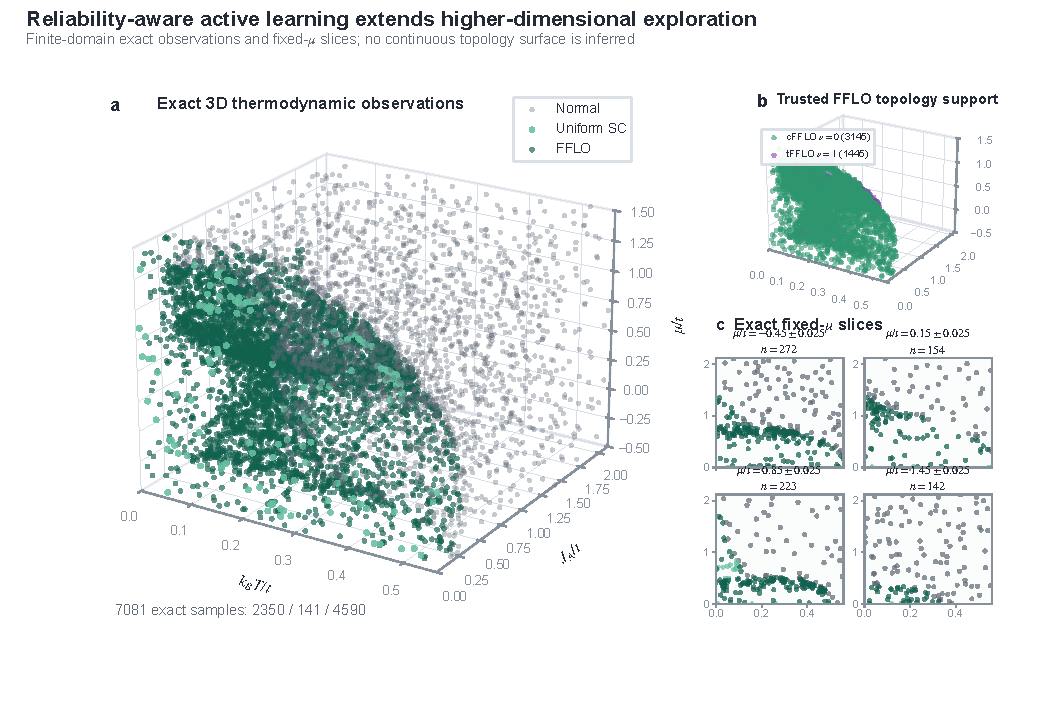
\includegraphics[width=0.98\columnwidth]{figures/Fig4_candidate.pdf}
\caption{\textbf{Finite-domain three-dimensional exploration.} \textbf{(a)} Exact thermodynamic observations in $(k_BT/t,J_A/t,\mu/t)$. \textbf{(b)} Discrete trusted FFLO topology support. \textbf{(c)} Four registered fixed-$\mu$ bins without interpolation. Slice populations reflect adaptive sampling and are not phase-volume estimates; the four cuts do not define a continuous topological surface.}
\label{fig:3d}\end{figure}

The three-dimensional point cloud establishes the finite sampled domain and displays how exact thermodynamic and topology labels populate it; the narrow slices provide readable local cross-sections without imposing continuity between them.  Selective evaluation is especially useful in this enlarged candidate space because it can retain exact authority while directing calls toward changing structures.  Nevertheless, nonuniform sampling prevents phase counts from being interpreted as thermodynamic volumes, and four cuts cannot determine a continuous boundary or topology surface.  Figure~\ref{fig:3d} therefore demonstrates scalable higher-dimensional exploration and chemical-potential-dependent reorganization, not a complete three-dimensional atlas or a fully resolved new mechanism.

\FloatBarrier
